\chapter{Methods and Testing}

So far we've written programs that have only one method named \java{main}.
In this chapter, we'll show you how to organize programs into multiple methods.
%We'll learn how to trace the order in which a program runs.
We'll also take a look at the \java{Math} class, which provides methods for common mathematical operations.
Finally, we'll discuss strategies for incrementally developing and testing your code.

%At a conceptual level, a method represents a mathematical {\em function} or a general {\em procedure}.
%Regardless whether they return a value or not, methods enable you to break down a complex program into smaller units of code.


\section{Defining New Methods}
\label{adding_methods}

Some methods perform a computation and return a result.
%For example, \java{Math.sqrt(25)} computes and returns the value \java{5.0}.
For example, \java{nextDouble} reads input from the keyboard and returns it as a \java{double}.
Other methods, like \java{println}, carry out a sequence of actions without returning a result.
Java uses the keyword \java{void} to define such methods.

%The \java{main} method always begins with the words \java{public static void}.
%You can define other methods the same way:

\begin{code}
public static void newLine() {
    System.out.println();
}

public static void main(String[] args) {
    System.out.println("First line.");
    newLine();
    System.out.println("Second line.");
}
\end{code}

\index{public}
\index{invoke}
\index{void}
\index{type!void}

In this example, the \java{newLine} and \java{main} methods are both \java{public}, which means they can be {\bf invoked} (or ``called'') from other classes.
%They are both \java{static}, but we won't yet explain what that means.
And they are both \java{void}, which means that they don't return a result (in contrast to \java{nextDouble}).
The output of the program is:

\begin{stdout}
First line.

Second line.
\end{stdout}

Notice the extra space between the lines.
If we wanted more space between them, we could invoke the same method repeatedly.
Or we could write yet another method (named \java{threeLine}) that displays three blank lines.
%Pulling together the code from the previous section, the complete program looks like this:

\index{NewLine.java}

\begin{trinket}{NewLine.java}
public class NewLine {

    public static void newLine() {
        System.out.println();
    }

    public static void threeLine() {
        newLine();
        newLine();
        newLine();
    }

    public static void main(String[] args) {
        System.out.println("First line.");
        threeLine();
        System.out.println("Second line.");
    }
}
\end{trinket}

\index{main}
\index{case-sensitive}

In this example, the name of the class is \java{NewLine}.
By convention, class names begin with a capital letter.
\java{NewLine} contains three methods, \java{newLine}, \java{threeLine}, and \java{main}.
Remember that Java is case-sensitive, so \java{NewLine} and \java{newLine} are not the same.

\index{camel case}

By convention, method names begin with a lowercase letter and use ``camel case'', which is a cute name for \java{jammingWordsTogetherLikeThis}.
You can use any name you want for methods, except \java{main} or any of the Java keywords.

%In the following program, \java{main} invokes \java{threeLine}, and \java{threeLine} invokes \java{newLine} three times.
%Since \java{newLine} has no parameters, it requires no arguments, as shown when it is invoked in \java{main}.
%Because \java{newLine} is in the same class as \java{threeLine}, we don't have to specify the class name like \java{NewLine.newLine()}.


\section{Flow of Execution}

\index{flow of execution}

When you look at a class definition that contains several methods, it is tempting to read it from top to bottom.
But that is {\em not} the {\bf flow of execution}, or the order the program actually runs.
The \java{NewLine} program runs methods in the opposite order than they are listed.

Programs always begin at the first statement of \java{main}, regardless of where it is in the source file.
Statements are executed one at a time, in order, until you reach a method invocation, which you can think of as a detour.
Instead of going to the next statement, you jump to the first line of the invoked method, execute all the statements there, and then come back and pick up exactly where you left off.

That sounds simple enough, but remember that one method can invoke another one.
In the middle of \java{main}, the previous example goes off to execute the statements in \java{threeLine}.
While in \java{threeLine}, it goes off to execute \java{newLine}.
Then \java{newLine} invokes \java{println}, which causes yet another detour.

Fortunately, Java is good at keeping track of which methods are running.
So when \java{println} completes, it picks up where it left off in \java{newLine}; when \java{newLine} completes, it goes back to \java{threeLine}; and when \java{threeLine} completes, it gets back to \java{main}.

%In summary, when you read a program, don't read from top to bottom.
%Instead, follow the flow of execution.

%Technically, the program does not terminate at the end of \java{main}.
%Instead, execution picks up where it left off in the program that invoked \java{main}, which is the Java interpreter.
%The interpreter takes care of things like deleting windows and general cleanup, and {\em then} the program terminates.

Beginners often wonder why it's worth the trouble to write other methods, when they could just do everything in \java{main}.
The \java{NewLine} example demonstrates a few reasons:

\begin{itemize}

\item Creating a new method allows you to {\em name a block of statements}, which makes the code easier to read and understand.
%Methods simplify a program by hiding complex computations behind a single statement, and by using English words in place of arcane code.
%Which is clearer, \java{newLine} or \java{System.out.println()}?

\item Introducing new methods can {\em make the program shorter} by eliminating repetitive code.
For example, to display nine consecutive newlines, you could invoke \java{threeLine} three times.

\item A common problem-solving technique is to {\em break problems down} into sub-problems.
Methods allow you to focus on each sub-problem in isolation, and then compose them into a complete solution.

\end{itemize}

Perhaps most importantly, organizing your code into multiple methods allows you to test individual parts of your program separately.
It's easier to get a complex program working if you know that each method works correctly.


\section{Parameters and Arguments}

Some of the methods we have used require {\bf arguments}, which are the values you provide in parentheses when you invoke the method.

%For example, the \java{Math.sin} method takes a \java{double} argument.
%To find the sine of a number, you have to provide the number: \java{Math.sin(0.0)}.

For example, the \java{println} method takes a \java{String} argument.
To display a message, you have to provide the message: \java{System.out.println("Hello")}.
Similarly, the \java{printf} method can take multiple arguments.
The statement \java{System.out.printf("\%d in = \%f cm\\n", inch, cm)} has three arguments: the format string, the \java{inch} value, and the \java{cm} value.


\index{parameter}
\index{argument}

When you invoke a method, you provide the arguments.
When you define a method, you name the {\bf parameters}, which are variables that indicate what arguments are required.
The following class shows an example:

\index{PrintTwice.java}

\begin{trinket}[295]{PrintTwice.java}
public class PrintTwice {

    public static void printTwice(String s) {
        System.out.println(s);
        System.out.println(s);
    }

    public static void main(String[] args) {
        printTwice("Don't make me say this twice!");
    }
}
\end{trinket}

The \java{printTwice} method has a parameter named \java{s} with type \java{String}.
When you invoke \java{printTwice}, you have to provide an argument with type \java{String}.

%\java{main} has a single parameter, called \java{args}, which has type \java{String[]}.
%That means that whoever invokes \java{main} must provide an array of strings (we'll get to arrays in a later chapter).

Before the method executes, the argument gets assigned to the parameter.
In the \java{printTwice} example, the argument \java{"Don't make me say this twice!"} gets assigned to the parameter \java{s}.

\index{parameter passing}

This process is called {\bf parameter passing}, because the value gets passed from outside the method to the inside.
An argument can be any kind of expression, so if you have a \java{String} variable, you can use its value as an argument:

\begin{code}
String message = "Never say never.";
printTwice(message);
\end{code}

The value you provide as an argument must have the same (or compatible) type as the parameter.
For example, if you try:

\begin{code}
printTwice(17);  // syntax error
\end{code}

You will get an error message like this:

\begin{stdout}
File: Test.java  [line: 10]
Error: method printTwice in class Test cannot be applied
       to given types;
  required: java.lang.String
  found: int
  reason: actual argument int cannot be converted to
          java.lang.String by method invocation conversion
\end{stdout}

This error message says that it found an \java{int} argument, but the required parameter should be a \java{String}.
In the case of \java{printTwice}, Java won't convert the integer \java{17} to the string \java{"17"} automatically.

\index{automatic conversion}

Sometimes Java can convert an argument from one type to another automatically.
For example, \java{Math.sqrt} requires a \java{double}, but if you invoke \java{Math.sqrt(25)}, the integer value \java{25} is automatically converted to the floating-point value \java{25.0}.

\index{local variable}
\index{variable!local}

Parameters and other variables only exist inside their own methods.
In the \java{printTwice} example, there is no such thing as \java{s} in the \java{main} method.
If you try to use it there, you'll get a compiler error.

Similarly, inside \java{printTwice} there is no such thing as \java{message}.
That variable belongs to \java{main}.
Because variables only exist inside the methods where they are defined, they are often called {\bf local variables}.


\section{Multiple Parameters}
\label{multparam}

\index{parameter!multiple}
\index{method!parameters}

Here is an example of a method that takes two parameters:

\begin{code}
public static void printTime(int hour, int minute) {
    System.out.print(hour);
    System.out.print(":");
    System.out.println(minute);
}
\end{code}

%In the parameter list, it may be tempting to write:
%
%\begin{code}
%public static void printTime(int hour, minute) {  // error
%\end{code}
%
%But that format (without the second \java{int}) is only allowed for local variables.
%For parameters, you need to declare the type of each variable separately.

To invoke this method, we have to provide two integers as arguments:

\begin{code}
int hour = 11;
int minute = 59;
printTime(hour, minute);
\end{code}

Beginners sometimes make the mistake of ``declaring'' the arguments:

\begin{code}
int hour = 11;
int minute = 59;
printTime(int hour, int minute);  // syntax error
\end{code}

That's a syntax error, because the compiler sees \java{int hour} and \java{int minute} as variable declarations, not expressions that represent values.
You wouldn't declare the types of the arguments if they were simply integers:

\begin{code}
printTime(int 11, int 59);  // syntax error
\end{code}

Pulling together the code fragments, here is the complete program:

\index{PrintTime.java}

\begin{trinket}[340]{PrintTime.java}
public class PrintTime {

    public static void printTime(int hour, int minute) {
        System.out.print(hour);
        System.out.print(":");
        System.out.println(minute);
    }

    public static void main(String[] args) {
        int hour = 11;
        int minute = 59;
        printTime(hour, minute);
    }
}
\end{trinket}

\java{printTime} has two parameters, named \java{hour} and \java{minute}.
And \java{main} has two variables, also named \java{hour} and \java{minute}.
Although they have the same names, these variables are {\em not} the same.
The \java{hour} in \java{printTime} and the \java{hour} in \java{main} refer to different memory locations, and they can have different values.
For example, you could invoke \java{printTime} like this:

\begin{code}
int hour = 11;
int minute = 59;
printTime(hour + 1, 0);
\end{code}

Before the method is invoked, Java evaluates the arguments; in this example, the results are \java{12} and \java{0}.
Then it assigns those values to the parameters.
Inside \java{printTime}, the value of \java{hour} is \java{12}, not \java{11}, and the value of \java{minute} is \java{0}, not \java{59}.
Furthermore, if \java{printTime} modifies one of its parameters, that change has no effect on the variables in \java{main}.


\section{Stack Diagrams}
\label{stack}

\index{stack diagram}
\index{diagram!stack}
\index{frame}

One way to keep track of variables is to draw a {\bf stack diagram}, which is a memory diagram (see Section~\ref{state}) that shows currently running methods.
For each method there is a box, called a {\bf frame}, that contains the method's parameters and local variables.
The name of the method appears outside the frame; the variables and parameters appear inside.

\begin{figure}[!ht]
\begin{center}
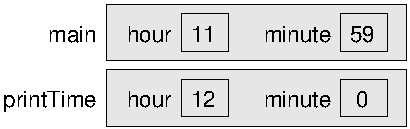
\includegraphics{figs/stack1.pdf}
\caption{Stack diagram for \java{printTime(hour + 1, 0)}.}
\label{fig.stack}
\end{center}
\end{figure}

As with memory diagrams, stack diagrams show variables and methods at a particular point in time.
Figure~\ref{fig.stack} is a stack diagram at the beginning of the \java{printTime} method.
Notice that \java{main} is on top, because it executed first.

\index{scope}

Stack diagrams help you to visualize the {\bf scope} of a variable, which is the area of a program where a variable can be used.

\index{Java Tutor}
\index{tracing}

Stack diagrams are a good mental model for how variables and methods work at run-time.
Learning to trace the execution of a program on paper (or on a whiteboard) is a useful skill for communicating with other programmers.

There are educational tools that automatically draw stack diagrams for you.
For example, Java Tutor (\url{https://thinkjava.org/javatutor}) allows you to step through an entire program, both forwards and backwards, and see the stack frames and variables at each step.
If you haven't already, you should check out the Java examples on that website.

%Or you can use a ``debugger'', like the one that comes with DrJava (see Appendix~\ref{debugger}).
%These tools also allow you to visualize the flow of execution.


\section{Math Methods}
\label{mathmeth}

\index{Math class}
\index{class!Math}

You don't always have to write new methods to get work done.
As a reminder, the Java library contains thousands of classes you can use.
For example, the \java{Math} class provides common mathematical operations.

\begin{code}
double root = Math.sqrt(17.0);
double angle = 1.5;
double height = Math.sin(angle);
\end{code}

The first line sets \java{root} to the square root of 17.
The third line finds the sine of 1.5 (the value of \java{angle}).
\java{Math} is in the \java{java.lang} package, so you don't have to import it.

\index{degrees}
\index{radians}
\index{pi}

Values for the trigonometric functions---\java{sin}, \java{cos}, and \java{tan}---must be in {\em radians}.
To convert from degrees to radians, you can divide by 180 and multiply by $\pi$.
Conveniently, the \java{Math} class provides a constant named \java{PI} that contains an approximation of $\pi$:

\begin{code}
double degrees = 90;
double angle = degrees / 180.0 * Math.PI;
\end{code}

Notice that \java{PI} is in capital letters.
Java does not recognize \java{Pi}, \java{pi}, or \java{pie}.
Also, \java{PI} is the name of a constant, not a method, so it doesn't have parentheses.
The same is true for the constant \java{Math.E}, which approximates Euler's number.

Converting to and from radians is a common operation, so the \java{Math} class provides methods that do that for you.

\begin{code}
double radians = Math.toRadians(180.0);
double degrees = Math.toDegrees(Math.PI);
\end{code}

\index{long}
\index{type!long}

Another useful method is \java{round}, which rounds a floating-point value to the nearest integer and returns a \java{long}.
The following result is 63 (rounded up from 62.8319).

\begin{code}
long x = Math.round(Math.PI * 20.0);
\end{code}

A \java{long} is like an \java{int}, but bigger.
More specifically, an \java{int} uses 32 bits of memory; the largest value it can hold is $2^{31}-1$, which is about 2 billion.
A \java{long} uses 64 bits, so the largest value is $2^{63}-1$, which is about 9 quintillion.

Take a minute to read the documentation for these and other methods in the \java{Math} class.
The easiest way to find documentation for Java classes is to do a web search for ``Java'' and the name of the class.


\section{Composition}

\index{expression}
\index{argument}

You have probably learned how to evaluate simple expressions like $\sin(\pi/2)$ and $\log(1/x)$.
First, you evaluate the expression in parentheses, which is the argument of the function.
Then you can evaluate the function itself, either by hand or by punching it into a calculator.

This process can be applied repeatedly to evaluate more complex expressions like $\log(1/\sin(\pi/2))$.
First we evaluate the argument of the innermost function ($\pi/2 = 1.57$), then evaluate the function itself ($\sin(1.57) = 1.0$), and so on.

\index{composition}
\index{expression}

Just as with mathematical functions, Java methods can be {\bf composed} to solve complex problems.
That means you can use one method as part of another.
In fact, you can use any expression as an argument to a method, as long as the resulting value has the correct type:

\begin{code}
double x = Math.cos(angle + Math.PI / 2.0);
\end{code}

This statement divides \java{Math.PI} by two, adds the result to \java{angle}, and computes the cosine of the sum.
You can also take the result of one method and pass it as an argument to another:

\begin{code}
double x = Math.exp(Math.log(10.0));
\end{code}

In Java, the \java{log} method always uses base $e$.
So this statement finds the log base $e$ of 10, and then raises $e$ to that power.
The result gets assigned to \java{x}.

Some math methods take more than one argument.
For example, \java{Math.pow} takes two arguments and raises the first to the power of the second.
This line computes $2^{10}$ and assigns the value \java{1024.0} to the variable \java{x}:

\begin{code}
double x = Math.pow(2.0, 10.0);
\end{code}

When using \java{Math} methods, beginners often forget the word \java{Math}.
For example, if you just write \java{x = pow(2.0, 10.0)}, you will get a compiler error:

\begin{stdout}
File: Test.java  [line: 5]
Error: cannot find symbol
  symbol:   method pow(double,double)
  location: class Test
\end{stdout}

The message ``cannot find symbol'' is confusing, but the last two lines provide a useful hint.
The compiler is looking for a method named \java{pow} in the file \java{Test.java} (the file for this example).
If you don't specify a class name when referring to a method, the compiler looks in the current class by default.


\section{Return Values}

\index{void}

When you invoke a \java{void} method, the invocation is usually on a line all by itself.
For example:

\begin{code}
printTime(hour + 1, 0);
\end{code}

On the other hand, when you invoke a value-returning method, you have to do something with the return value.
We usually assign it to a variable or use it as part of an expression, like this:

\begin{code}
double error = Math.abs(expect - actual);
double height = radius * Math.sin(angle);
\end{code}

\index{value method}
\index{method!value}

Compared to \java{void} methods, value-returning methods differ in two ways:

\index{return type}
\index{return value}

\begin{itemize}

\item They declare the type of the return value (the {\bf return type});

\item They use at least one \java{return} statement to provide a {\bf return value}.

\end{itemize}

Here's an example from a program named {\tt Circle.java}.
The \java{calculateArea} method takes a \java{double} as a parameter and returns the area of a circle with that radius (i.e., $\pi r^2$).

\begin{code}
public static double calculateArea(double radius) {
    double result = Math.PI * radius * radius;
    return result;
}
\end{code}

As usual, this method is \java{public} and \java{static}.
But in the place where we are used to seeing \java{void}, we see \java{double}, which means that the return value from this method is a \java{double}.

\index{return}
\index{statement!return}

The last line is a new form of the \java{return} statement that means, ``return immediately from this method, and use the following expression as the return value.''
The expression you provide can be arbitrarily complex, so we could have written this method more concisely:

\begin{code}
public static double calculateArea(double radius) {
    return Math.PI * radius * radius;
}
\end{code}

\index{temporary variable}
\index{variable!temporary}

On the other hand, {\bf temporary variables} like \java{result} often make debugging easier, especially when you are stepping through code using an interactive debugger (see Appendix~\ref{debugger}).

Figure~\ref{fig.param} illustrates how data values flows through the program.
When the \java{main} method invokes \java{calculateArea}, the value \java{5.0} is assigned to the parameter \java{radius}.
\java{calculateArea} then returns the value \java{78.54}, which is assigned to the variable \java{area}.
%Note that you don't ``pass variables'' as arguments and return values---you copy their values.

\begin{figure}[!ht]
\begin{center}
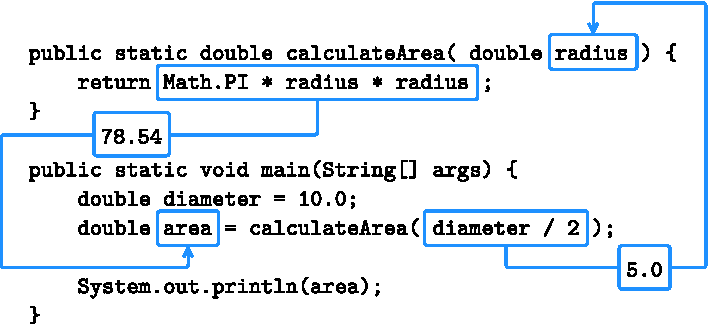
\includegraphics{figs/param.pdf}
\caption{Passing a parameter and saving the return value.}
\label{fig.param}
\end{center}
\end{figure}

The type of the expression in the \java{return} statement must match the return type of the method itself.
When you declare that the return type is \java{double}, you are making a promise that this method will eventually produce a \java{double} value.
If you try to \java{return} with no expression, or \java{return} an expression with the wrong type, the compiler will give an error.


\section{Incremental Development}
\label{distance}

\index{incremental development}
\index{design process}

People often make the mistake of writing a lot of code before they try to compile and run it.
Then they spend way too much time debugging.
A better approach is what we call {\bf incremental development}.
The key aspects of incremental development are:

\begin{itemize}

\item Start with a working program and make small, incremental changes.
At any point, if there is an error, you will know where to look.

\item Use variables to hold intermediate values so you can check them, either with print statements or by using a debugger.

\item Once the program is working, you can consolidate multiple statements into compound expressions (but only if it does not make the program more difficult to read).

\end{itemize}

As an example, suppose you want to find the distance between two points, given by the coordinates $(x_1, y_1)$ and $(x_2, y_2)$.
By the usual definition:

\[ distance = \sqrt{(x_2 - x_1)^2 +(y_2 - y_1)^2} \]

The first step is to consider what a \java{distance} method should look like in Java.
In other words, what are the inputs (parameters) and what is the output (return value)?
For this method, the parameters are the two points, and it is natural to represent them using four \java{double} values.
%, although we will see later that there is a \java{Point} object in Java that we could use.
The return value is the distance, which should also have type \java{double}.

\index{stub}

Already we can write an outline for the method, which is sometimes called a {\bf stub}.
The stub includes the method declaration and a \java{return} statement:

\begin{code}
public static double distance
        (double x1, double y1, double x2, double y2) {
    return 0.0;  // stub
}
\end{code}

The return statement is a placeholder that is only necessary for the program to compile.
At this stage the program doesn't do anything useful, but it is good to compile it so we can find any syntax errors before we add more code.

\index{testing}

It's usually a good idea to think about testing {\em before} you develop new methods; doing so can help you figure out how to implement them.
To test the method, we can invoke it from \java{main} using the sample values:

\begin{code}
double dist = distance(1.0, 2.0, 4.0, 6.0);
\end{code}

With these values, the horizontal distance is 3.0 and the vertical distance is 4.0.
So the result should be 5.0, the hypotenuse of a 3-4-5 triangle.
When you are testing a method, it is necessary to know the right answer.

Once we have compiled the stub, we can start adding code one line at a time.
After each incremental change, we recompile and run the program.
If there is an error, we have a good idea where to look: the lines we just added.

The next step is to find the differences $x_2 - x_1$ and $y_2 - y_1$.
We store those values in temporary variables named \java{dx} and \java{dy}, so that we can examine them with print statements before proceeding.
They should be 3.0 and 4.0.

\begin{code}
public static double distance
        (double x1, double y1, double x2, double y2) {
    double dx = x2 - x1;
    double dy = y2 - y1;
    System.out.println("dx is " + dx);
    System.out.println("dy is " + dy);
    return 0.0;  // stub
}
\end{code}

\index{scaffolding}

We will remove the print statements when the method is finished.
Code like that is called {\bf scaffolding}, because it is helpful for building the program, but it is not part of the final product.

The next step is to square \java{dx} and \java{dy}.
We could use the \java{Math.pow} method, but it is simpler (and more efficient) to multiply each term by itself.

Then we add the squares and print the result so far.

\begin{code}
public static double distance
        (double x1, double y1, double x2, double y2) {
    double dx = x2 - x1;
    double dy = y2 - y1;
    double dsquared = dx * dx + dy * dy;
    System.out.println("dsquared is " + dsquared);
    return 0.0;  // stub
}
\end{code}

Again, you should compile and run the program at this stage and check the intermediate value, which should be 25.0.
Finally, we can use \java{Math.sqrt} to compute and return the result.

\begin{code}
public static double distance
        (double x1, double y1, double x2, double y2) {
    double dx = x2 - x1;
    double dy = y2 - y1;
    double dsquared = dx * dx + dy * dy;
    double result = Math.sqrt(dsquared);
    return result;
}
\end{code}

%In \java{main}, we can print and check the value of the result.

As you gain more experience programming, you might write and debug more than one line at a time.
But if you find yourself spending a lot of time debugging, consider taking smaller steps.
%Nevertheless, incremental development can save you a lot of time debugging.
%But by using incremental development, scaffolding, and testing, your code is more likely to be correct the first time.


\section{Vocabulary}

\begin{description}

% Note: expanded definition from Chapter 1
%\term{method}
%A named sequence of statements that performs a procedure or function.
%Methods may or may not take parameters, and may or may not return a value.

\term{void}
A special return type indicating the method does not return a value.

\term{invoke}
To cause a method to execute.
Also known as ``calling'' a method.

\term{flow of execution}
The order in which Java executes methods and statements.
It may not necessarily be from top to bottom in the source file.

\term{argument}
A value that you provide when you call a method.
This value must have the type that the method expects.

\term{parameter}
A piece of information that a method requires before it can run.
Parameters are variables: they contain values and have types.

\term{parameter passing}
The process of assigning an argument value to a parameter variable.

\term{local variable}
A variable declared inside a method.
Local variables cannot be accessed from outside their method.

\term{stack diagram}
A graphical representation of the variables belonging to each method.
The method calls are ``stacked'' from top to bottom, in the flow of execution.

\term{frame}
In a stack diagram, a representation of the variables and parameters for a method, along with their current values.

\term{scope}
The area of a program where a variable can be used.

\term{composition}
The ability to combine simple expressions and statements into compound expressions and statements.

\term{return type}
The type of value a method returns.

\term{return value}
The value provided as the result of a method invocation.

\term{temporary variable}
A short-lived variable, often used for debugging.

\term{incremental development}
A process for creating programs by writing a few lines at a time, compiling, and testing.

\term{stub}
A placeholder for an incomplete method so that the class will compile.

\term{scaffolding}
Code that is used during program development but is not part of the final version.

\end{description}


\section{Exercises}

The code for this chapter is in the {\tt ch04} directory of {\tt ThinkJavaCode2}.
See page~\pageref{code} for instructions on how to download the repository.
Before you start the exercises, we recommend that you compile and run the examples.

If you have not already read Appendix~\ref{cltesting}, now might be a good time.
It describes an efficient way to test programs that take input from the user and display specific output.


\begin{exercise}  %%V6 Ex4.3

The purpose of this exercise is to take code from a previous exercise and redesign it as a method that takes parameters.
You should start with a working solution to Exercise~\ref{ex:date}.

\vspace{-1em}
\begin{enumerate}

\item Write a method called \java{printAmerican} that takes the day, date, month and year as parameters and that displays them in American format.

\item Test your method by invoking it from \java{main} and passing appropriate arguments.
The output should look something like this (except that the date might be different):

\begin{stdout}
Saturday, July 22, 2015
\end{stdout}

\item Once you have debugged \java{printAmerican}, write another method called \java{printEuropean} that displays the date in European format.

\end{enumerate}
\vspace{1ex}

\end{exercise}


\begin{exercise}  %%V6 Ex5.6

This exercise reviews the flow of execution through a program with multiple methods.
Read the following code and answer the questions.

\begin{code}
public static void main(String[] args) {
    zippo("rattle", 13);
}
\end{code}

\begin{code}
public static void baffle(String blimp) {
    System.out.println(blimp);
    zippo("ping", -5);
}
\end{code}

\begin{code}
public static void zippo(String quince, int flag) {
    if (flag < 0) {
        System.out.println(quince + " zoop");
    } else {
        System.out.println("ik");
        baffle(quince);
        System.out.println("boo-wa-ha-ha");
    }
}
\end{code}

\begin{enumerate}

\item Write the number {\tt 1} next to the first line of code in this program that will execute.

\item Write the number {\tt 2} next to the second line of code, and so on until the end of the program.
If a line is executed more than once, it might end up with more than one number next to it.

\item What is the value of the parameter \java{blimp} when \java{baffle} gets invoked?

\item What is the output of this program?

\end{enumerate}

\end{exercise}


\begin{exercise}  %%V6 Ex4.1

%The point of this exercise is to practice reading code and to make sure that you understand the flow of execution through a program with multiple methods.
Answer the following questions without running the program on a computer.

\begin{enumerate}

\item Draw a stack diagram that shows the state of the program the first time \java{ping} is invoked.

\item What is output by the following program?
Be precise about where there are spaces and where there are newlines.

%{\it Hint:} Start by describing in words what \java{ping} and \java{baffle} output.

%\item What happens if you invoke \java{baffle();} at the end of the \java{ping} method? (We will see why in Section~\ref{recursion}.)

\end{enumerate}

\begin{code}
public static void zoop() {
    baffle();
    System.out.print("You wugga ");
    baffle();
}
\end{code}

\begin{code}
public static void main(String[] args) {
    System.out.print("No, I ");
    zoop();
    System.out.print("I ");
    baffle();
}
\end{code}

\begin{code}
public static void baffle() {
    System.out.print("wug");
    ping();
}
\end{code}

\begin{code}
public static void ping() {
    System.out.println(".");
}
\end{code}

\end{exercise}


\begin{exercise}  %%V6 Ex6.1

If you have a question about whether something is legal, and what happens if it is not, a good way to find out is to ask the compiler.
Answer the following questions by trying them out.

\begin{enumerate}

\item What happens if you invoke a value method and don't do anything with the result; that is, if you don't assign it to a variable or use it as part of a larger expression?

\item What happens if you use a void method as part of an expression?
For example, try \java{System.out.println("boo!") + 7;}

\end{enumerate}

\end{exercise}


\begin{exercise}  %%V6 Ex5.2

Draw a stack diagram that shows the state of the program the {\it second} time \java{zoop} is invoked.
What is the complete output?

\begin{code}
public static void zoop(String fred, int bob) {
    System.out.println(fred);
    if (bob == 5) {
        ping("not ");
    } else {
        System.out.println("!");
    }
}
\end{code}

\begin{code}
public static void main(String[] args) {
    int bizz = 5;
    int buzz = 2;
    zoop("just for", bizz);
    clink(2 * buzz);
}
\end{code}

\begin{code}
public static void clink(int fork) {
    System.out.print("It's ");
    zoop("breakfast ", fork);
}
\end{code}

\begin{code}
public static void ping(String strangStrung) {
    System.out.println("any " + strangStrung + "more ");
}
\end{code}

\end{exercise}


\begin{exercise}  %%V6 Ex6.4

Many computations can be expressed more concisely using the ``multadd'' operation, which takes three operands and computes \java{a * b + c}.
Some processors even provide a hardware implementation of this operation for floating-point numbers.

\begin{enumerate}

\item Create a new program called {\tt Multadd.java}.

\item Write a method called \java{multadd} that takes three \java{doubles} as parameters and that returns \java{a * b + c}.

\item Write a \java{main} method that tests \java{multadd} by invoking it with a few simple parameters, like \java{1.0, 2.0, 3.0}.

\item Also in \java{main}, use \java{multadd} to compute the following values:
%
\begin{eqnarray*}
& \sin \frac{\pi}{4} + \frac{\cos \frac{\pi}{4}}{2} & \\
& \log 10 + \log 20 &
\end{eqnarray*}

\item Write a method called \java{expSum} that takes a double as a parameter and that uses \java{multadd} to calculate:
%
\begin{eqnarray*}
x e^{-x} + \sqrt{1 - e^{-x}}
\end{eqnarray*}
%
{\it Hint:} The method for raising $e$ to a power is \java{Math.exp}.

\end{enumerate}

In the last part of this exercise, you need to write a method that invokes another method you wrote.
Whenever you do that, it is a good idea to test the first method carefully before working on the second.
Otherwise, you might find yourself debugging two methods at the same time, which can be difficult.

One of the purposes of this exercise is to practice pattern-matching: the ability to recognize a specific problem as an instance of a general category of problems.

\end{exercise}
